\section{Tecnologie - Transazioni}
\subsection{Tecnologia dei DBMS}
Un \textbf{DBMS} (Database Management System), o \textit{sistema di gestione di basi di dati}, 
è un sistema software progettato per gestire collezioni di dati che siano:

\begin{itemize}
	\item \textbf{Grandi} (di dimensioni tali da richiedere gestione su memoria secondaria);
	\item \textbf{Condivise} (accessibili da più utenti o applicazioni contemporaneamente);
	\item \textbf{Persistenti} (i dati sopravvivono all'esecuzione dei programmi che li utilizzano).
\end{itemize}

Un DBMS garantisce:
\begin{itemize}
	\item \textbf{Affidabilità} (integrità e recupero dei dati in caso di guasti);
	\item \textbf{Privatezza e sicurezza} (controllo degli accessi e gestione dei permessi).
\end{itemize}

Essendo un sistema software, un DBMS deve essere:
\begin{itemize}
	\item \textbf{Efficiente}, ottimizzando l’uso delle risorse (tempo di risposta e spazio);
	\item \textbf{Efficace}, fornendo strumenti adeguati per la gestione e l’organizzazione dei dati.
\end{itemize}

Le prestazioni e la qualità complessiva del sistema dipendono in modo significativo 
dalla \textbf{corretta progettazione della base di dati}.

Un DBMS:
\begin{itemize}
	\item Estende le funzionalità del \textit{file system};
	\item Gestisce collezioni di dati memorizzate in \textbf{memoria secondaria};
	\item Fornisce meccanismi di accesso, manipolazione e controllo dei dati.
\end{itemize}

\textbf{Base di dati:} una collezione organizzata di dati, gestita e controllata da un DBMS.
\subsection{Architettura su 3 livelli dei DBMS}
\begin{figure}[H]
	\centering
	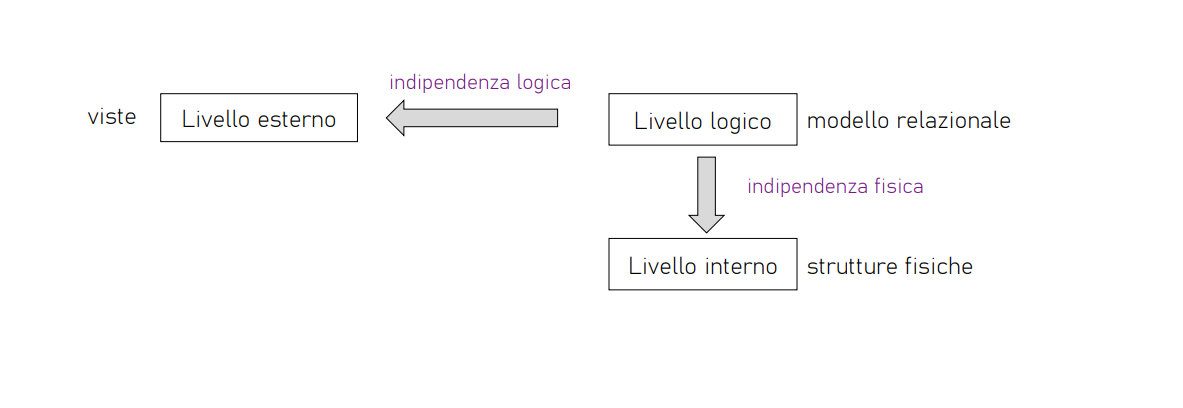
\includegraphics[width=1\linewidth]{image106}
	\caption{Architettura su 3 livelli dei DBMS}
	\label{fig:image106}
\end{figure}

Un DBMS è organizzato secondo un'architettura a tre livelli: \textbf{esterno}, \textbf{logico} e \textbf{interno}. 
Il \textbf{livello esterno} descrive le viste degli utenti: ad esempio, uno studente può visualizzare solo i propri voti, mentre la segreteria può accedere ai dati di tutti gli studenti. 
Il \textbf{livello logico} definisce la struttura concettuale della base di dati nel modello relazionale, ad esempio la tabella \texttt{Studenti(Matricola, Nome, Cognome, Corso)}, indipendentemente dalla memorizzazione fisica. 
Il \textbf{livello interno}, infine, descrive come i dati sono effettivamente memorizzati su disco, ad esempio in file organizzati in pagine con eventuali indici per ottimizzare le ricerche.

Questa separazione garantisce l'\textbf{indipendenza logica}, per cui modifiche allo schema logico non richiedono cambiamenti nelle viste esterne, e l'\textbf{indipendenza fisica}, per cui variazioni nell'organizzazione fisica dei dati non alterano lo schema logico.
\subsection{Transazione}
Una \textbf{transazione} è un'unità logica di lavoro eseguita da un programma applicativo che interagisce con una base di dati. 
È costituita da una sequenza di operazioni che devono essere considerate come un unico blocco indivisibile.

Una transazione deve garantire proprietà di \textbf{correttezza}, \textbf{robustezza} e \textbf{isolamento}, in modo da mantenere la consistenza della base di dati anche in presenza di errori o accessi concorrenti.

La caratteristica fondamentale di una transazione è il principio \textit{all-or-nothing}: 
essa o termina con successo (\textbf{commit}) producendo effetti permanenti sulla base di dati, oppure viene annullata (\textbf{abort/rollback}) senza lasciare alcuna modifica. 
\begin{figure}[H]
	\centering
	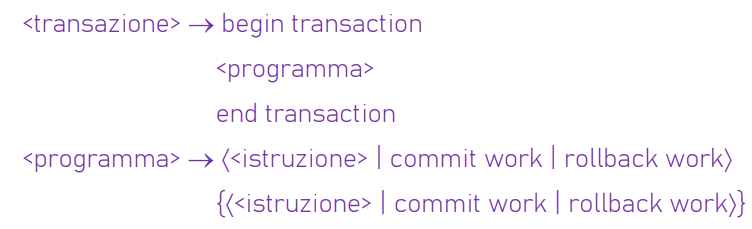
\includegraphics[width=1\linewidth]{image107}
	\caption{Sintassi di una transazione}
	\label{fig:image107}
\end{figure}
Una \textbf{transazione} si dice \emph{ben formata} se rispetta le seguenti condizioni:

\begin{itemize}
	\item Inizia esplicitamente con un'istruzione \texttt{BEGIN TRANSACTION}.
	
	\item Termina con un'istruzione \texttt{END TRANSACTION}.
	
	\item Durante la sua esecuzione viene raggiunto un punto di terminazione esplicito, 
	ovvero un'istruzione \texttt{COMMIT WORK} oppure \texttt{ROLLBACK WORK}.
	
	\item Dopo l'esecuzione di \texttt{COMMIT} o \texttt{ROLLBACK} non vengono effettuati 
	ulteriori accessi o modifiche alla base di dati all'interno della stessa transazione.
\end{itemize}
\begin{figure}[H]
	\centering
	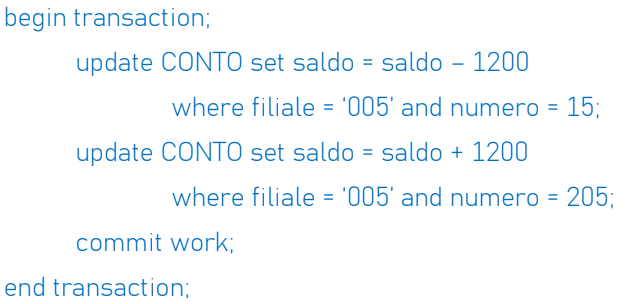
\includegraphics[width=1\linewidth]{image108}
	\caption{Esempio transazione ben formata}
	\label{fig:image108}
\end{figure}
\subsubsection{Proprietà delle transazioni}
Una transazione in un DBMS deve rispettare quattro proprietà fondamentali,
note come proprietà \textbf{ACID}:

\begin{itemize}
	
	\item \textbf{Atomicità (Atomicity)}: una transazione è un'unità di esecuzione indivisibile. 
	Essa viene eseguita completamente oppure non viene eseguita affatto.
	
	Implicazioni:
	\begin{itemize}
		\item Se una transazione viene interrotta prima del \texttt{commit}, il lavoro eseguito fino a quel momento deve essere annullato, ripristinando lo stato della base di dati precedente all'inizio della transazione.
		
		\item Se una transazione viene interrotta dopo l'esecuzione del \texttt{commit} (commit completato con successo), il sistema deve garantire che gli effetti della transazione siano permanentemente registrati nella base di dati.
	\end{itemize}
	
	\item \textbf{Consistenza (Consistency)}: l'esecuzione di una transazione non deve violare i vincoli di integrità della base di dati.
	
	Implicazioni:
	\begin{itemize}
		\item \textbf{Verifica immediata}: il controllo dei vincoli viene effettuato durante l'esecuzione della transazione. Se un vincolo viene violato, viene annullata solo l'ultima operazione eseguita e il sistema restituisce all'applicazione una segnalazione di errore. L'applicazione può quindi reagire alla violazione.
		
		\item \textbf{Verifica differita}: il controllo dei vincoli viene effettuato al momento del \texttt{commit}. Se un vincolo di integrità risulta violato, l'intera transazione viene abortita senza possibilità per l'applicazione di reagire alla violazione.
	\end{itemize}
	
	\item \textbf{Isolamento (Isolation)}: l'esecuzione di una transazione deve essere indipendente dalla contemporanea esecuzione di altre transazioni.
	
	Implicazioni:
	\begin{itemize}
		\item Il rollback di una transazione non deve causare rollback a catena di altre transazioni che si trovano in esecuzione contemporaneamente.
		
		\item Il sistema deve regolare l'esecuzione concorrente tramite meccanismi di controllo dell'accesso alle risorse.
	\end{itemize}
	
	\item \textbf{Persistenza (Durability)}: l'effetto di una transazione che ha eseguito il \texttt{commit} non deve andare perso.
	
	Implicazioni:
	\begin{itemize}
		\item Il sistema deve essere in grado, in caso di guasto, di garantire gli effetti delle transazioni che al momento del guasto avevano già eseguito un \texttt{commit}.
	\end{itemize}
	
\end{itemize}
\subsection{Architettura di un DBMS}
Un DBMS è composto da diversi moduli che gestiscono le varie funzionalità
necessarie all'esecuzione delle transazioni.
\begin{figure}[H]
	\centering
	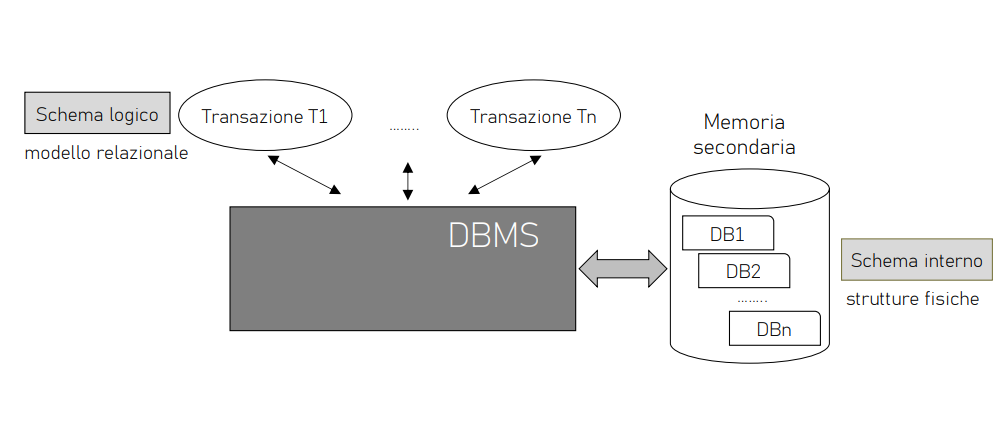
\includegraphics[width=1\linewidth]{image109}
	\caption{Architettura di riferimento di un DBMS}
	\label{fig:image109}
\end{figure}
La figura rappresenta l'interazione tra le transazioni degli utenti, il DBMS e la
memoria secondaria. Le transazioni (T1, \ldots, Tn) operano sullo \textbf{schema
	logico} del database secondo il modello relazionale e inviano le loro operazioni
al DBMS. Il \textbf{DBMS} funge da intermediario, gestendo l'esecuzione delle
transazioni e garantendo le proprietà di correttezza del sistema. I dati sono
memorizzati nella \textbf{memoria secondaria} (DB1, DB2, \ldots, DBn) secondo lo
\textbf{schema interno}, che descrive le strutture fisiche utilizzate per
organizzare e memorizzare i dati.
\begin{figure}[H]
	\centering
	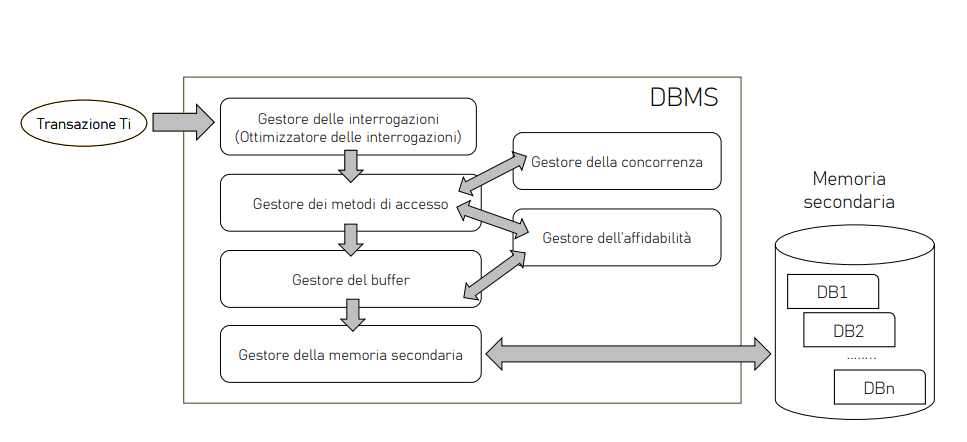
\includegraphics[width=1\linewidth]{image110}
	\caption{Moduli principali di un DBMS}
	\label{fig:image110}
\end{figure}
La figura mostra i principali moduli che compongono l'architettura interna di un
DBMS e il modo in cui collaborano durante l'esecuzione di una transazione.

Una transazione $T_i$ invia le proprie interrogazioni al \textbf{gestore delle
	interrogazioni} (query processor), che analizza e ottimizza le query per
determinare il piano di esecuzione più efficiente. Il \textbf{gestore dei metodi
	di accesso} stabilisce come accedere ai dati, utilizzando strutture come indici
o scansioni delle tabelle.

Il \textbf{gestore del buffer} si occupa della gestione delle pagine di dati in
memoria principale, mentre il \textbf{gestore della memoria secondaria} gestisce
l'accesso fisico ai dati memorizzati su disco.

Il \textbf{gestore della concorrenza} controlla l'esecuzione simultanea di più
transazioni per evitare interferenze, mentre il \textbf{gestore
	dell'affidabilità} garantisce la correttezza delle operazioni anche in caso di
guasti, assicurando il mantenimento delle proprietà ACID.
\begin{figure}[H]
	\centering
	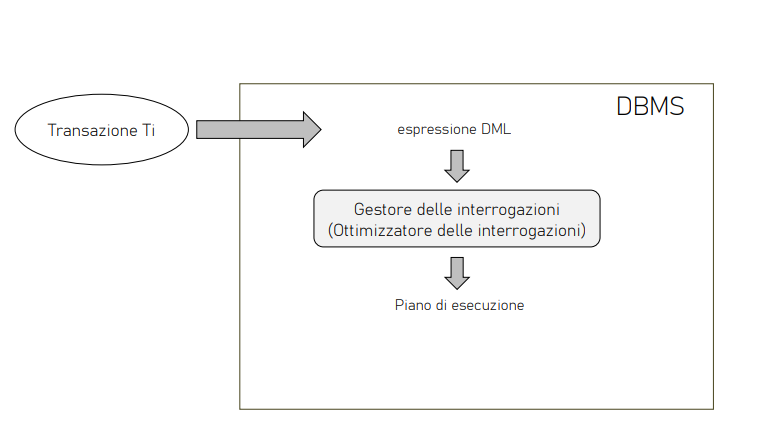
\includegraphics[width=1\linewidth]{image111}
	\caption{fase di elaborazione di una query}
	\label{fig:image111}
\end{figure}
Una transazione $T_i$ invia al DBMS un'espressione del linguaggio DML.
La query viene elaborata dal \textbf{gestore delle interrogazioni}
(query processor), che analizza e ottimizza l'interrogazione.
Il risultato di questo processo è un \textbf{piano di esecuzione},
ovvero una sequenza di operazioni che il DBMS esegue per ottenere
il risultato richiesto in modo efficiente.
\begin{figure}[H]
	\centering
	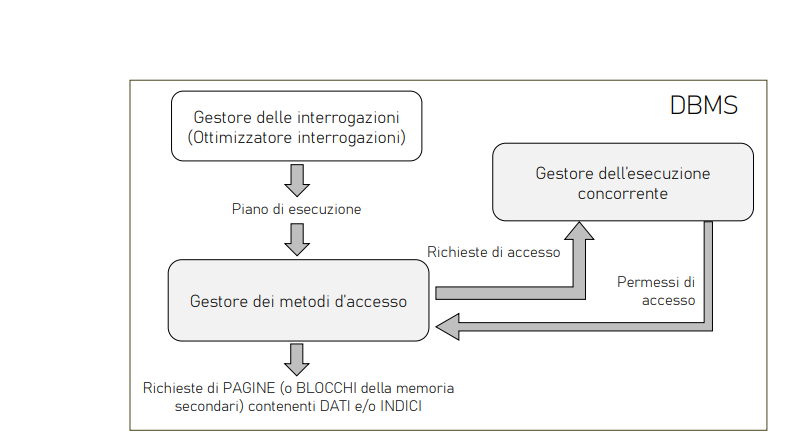
\includegraphics[width=1\linewidth]{image112}
	\caption{gestione delle interrogazioni}
	\label{fig:image112}
\end{figure}
Il piano di esecuzione prodotto dal gestore delle interrogazioni viene
eseguito dal gestore dei metodi di accesso, che richiede le pagine di
dati o indici dalla memoria secondaria. Le richieste di accesso ai dati
vengono controllate dal gestore dell'esecuzione concorrente, che verifica
la compatibilità con le altre transazioni in esecuzione e concede i
permessi di accesso. In questo modo il DBMS garantisce l'esecuzione
corretta delle transazioni concorrenti.
\begin{figure}[H]
	\centering
	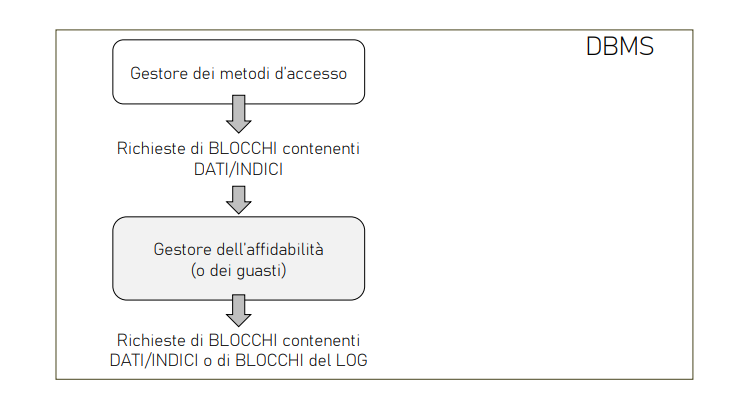
\includegraphics[width=1\linewidth]{image113}
	\caption{fase di recovery}
	\label{fig:image113}
\end{figure}
Le richieste di accesso ai blocchi contenenti dati o indici, generate dal
gestore dei metodi di accesso, vengono gestite dal \textbf{gestore
	dell'affidabilità} (recovery manager). Questo modulo ha il compito di
garantire la correttezza del database anche in caso di guasti,
utilizzando il \textbf{log delle transazioni}. Il log registra le
operazioni eseguite dalle transazioni e permette al sistema di
ripristinare lo stato corretto della base di dati attraverso operazioni
di \emph{redo} e \emph{undo}.
\begin{figure}[H]
	\centering
	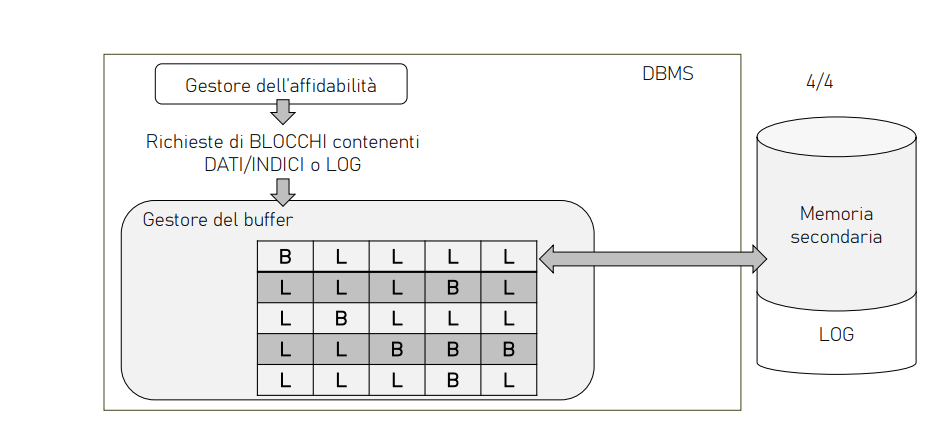
\includegraphics[width=1\linewidth]{image114}
	\caption{fase di gestione della memoria principale tramite il buffer manager quando accede ai dati sul disco}
	\label{fig:image114}
\end{figure}
Le richieste di accesso ai blocchi contenenti dati, indici o record del log,
generate dal gestore dell'affidabilità, vengono gestite dal
\textbf{gestore del buffer}. Questo modulo mantiene in memoria principale
una copia delle pagine utilizzate più frequentemente, riducendo gli
accessi alla memoria secondaria. Quando necessario, il buffer manager
carica nuove pagine dal disco o scrive sul disco le pagine modificate.
\begin{figure}[H]
	\centering
	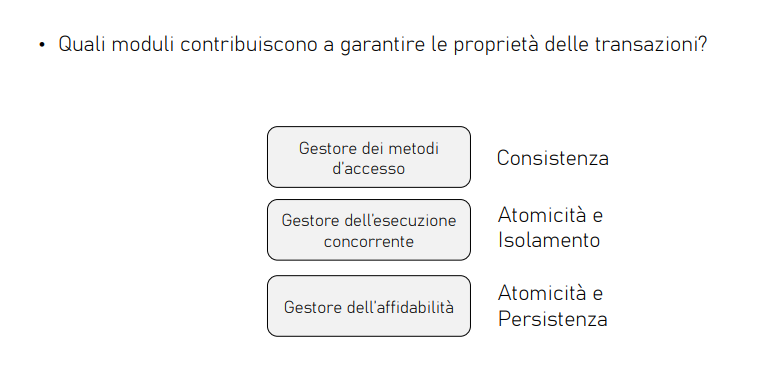
\includegraphics[width=1\linewidth]{image115}
	\caption{}
	\label{fig:image115}
\end{figure}
